\ifdefined\included
\else
\setcounter{chapter}{6} %% Numéro du chapitre précédent ;)
\dominitoc
\faketableofcontents
\fi

\chapter{Extending the REG with knowledge about past activities}
\chaptermark{REG with knowledge about past activities}
\minitoc

The contribution presented in this chapter is excerpted from our work, submited to the IROS 2021 conference. In this manuscript, the contribution is more detailed and discussed. In the continuity of the two previous, the presented work has been achieved in collaboration with Guilhem Buisan. He brought his expertise on HTNs to allow the best possible representation in an ontology.

\section{Introduction}

When two or more agents perform a collaborative task, although they may have a different perception of their shared environment, they can estimate the information they share and can thus use it to communicate about entities they estimated to be known by the others. This assumption is the one commonly used to develop and evaluate Referring Expression Generation (REG) methods through the use of caption of the environment\cite{duboue_2015_evaluating}. These captions are images always took from the hearer point of view. The image, or the related knowledge representation, is provided to the algorithm which has to generate a referring expression. This assumption has also been used when the REG has been applied to Human-Robot Interaction (HRI) and can be compared to a robot spawning in an environment and having to designate an object. However, this designation occurs during a joint activity between a robot and a human partner meaning that the designated objects may have been used, moved, or already speak about. All of this information about the performed task can be seen as additional knowledge shared by the involved agents. We can thus refer to the entities through these past actions in addition to their attributes and relations with each other.

\begin{figure}[ht!]
\centering
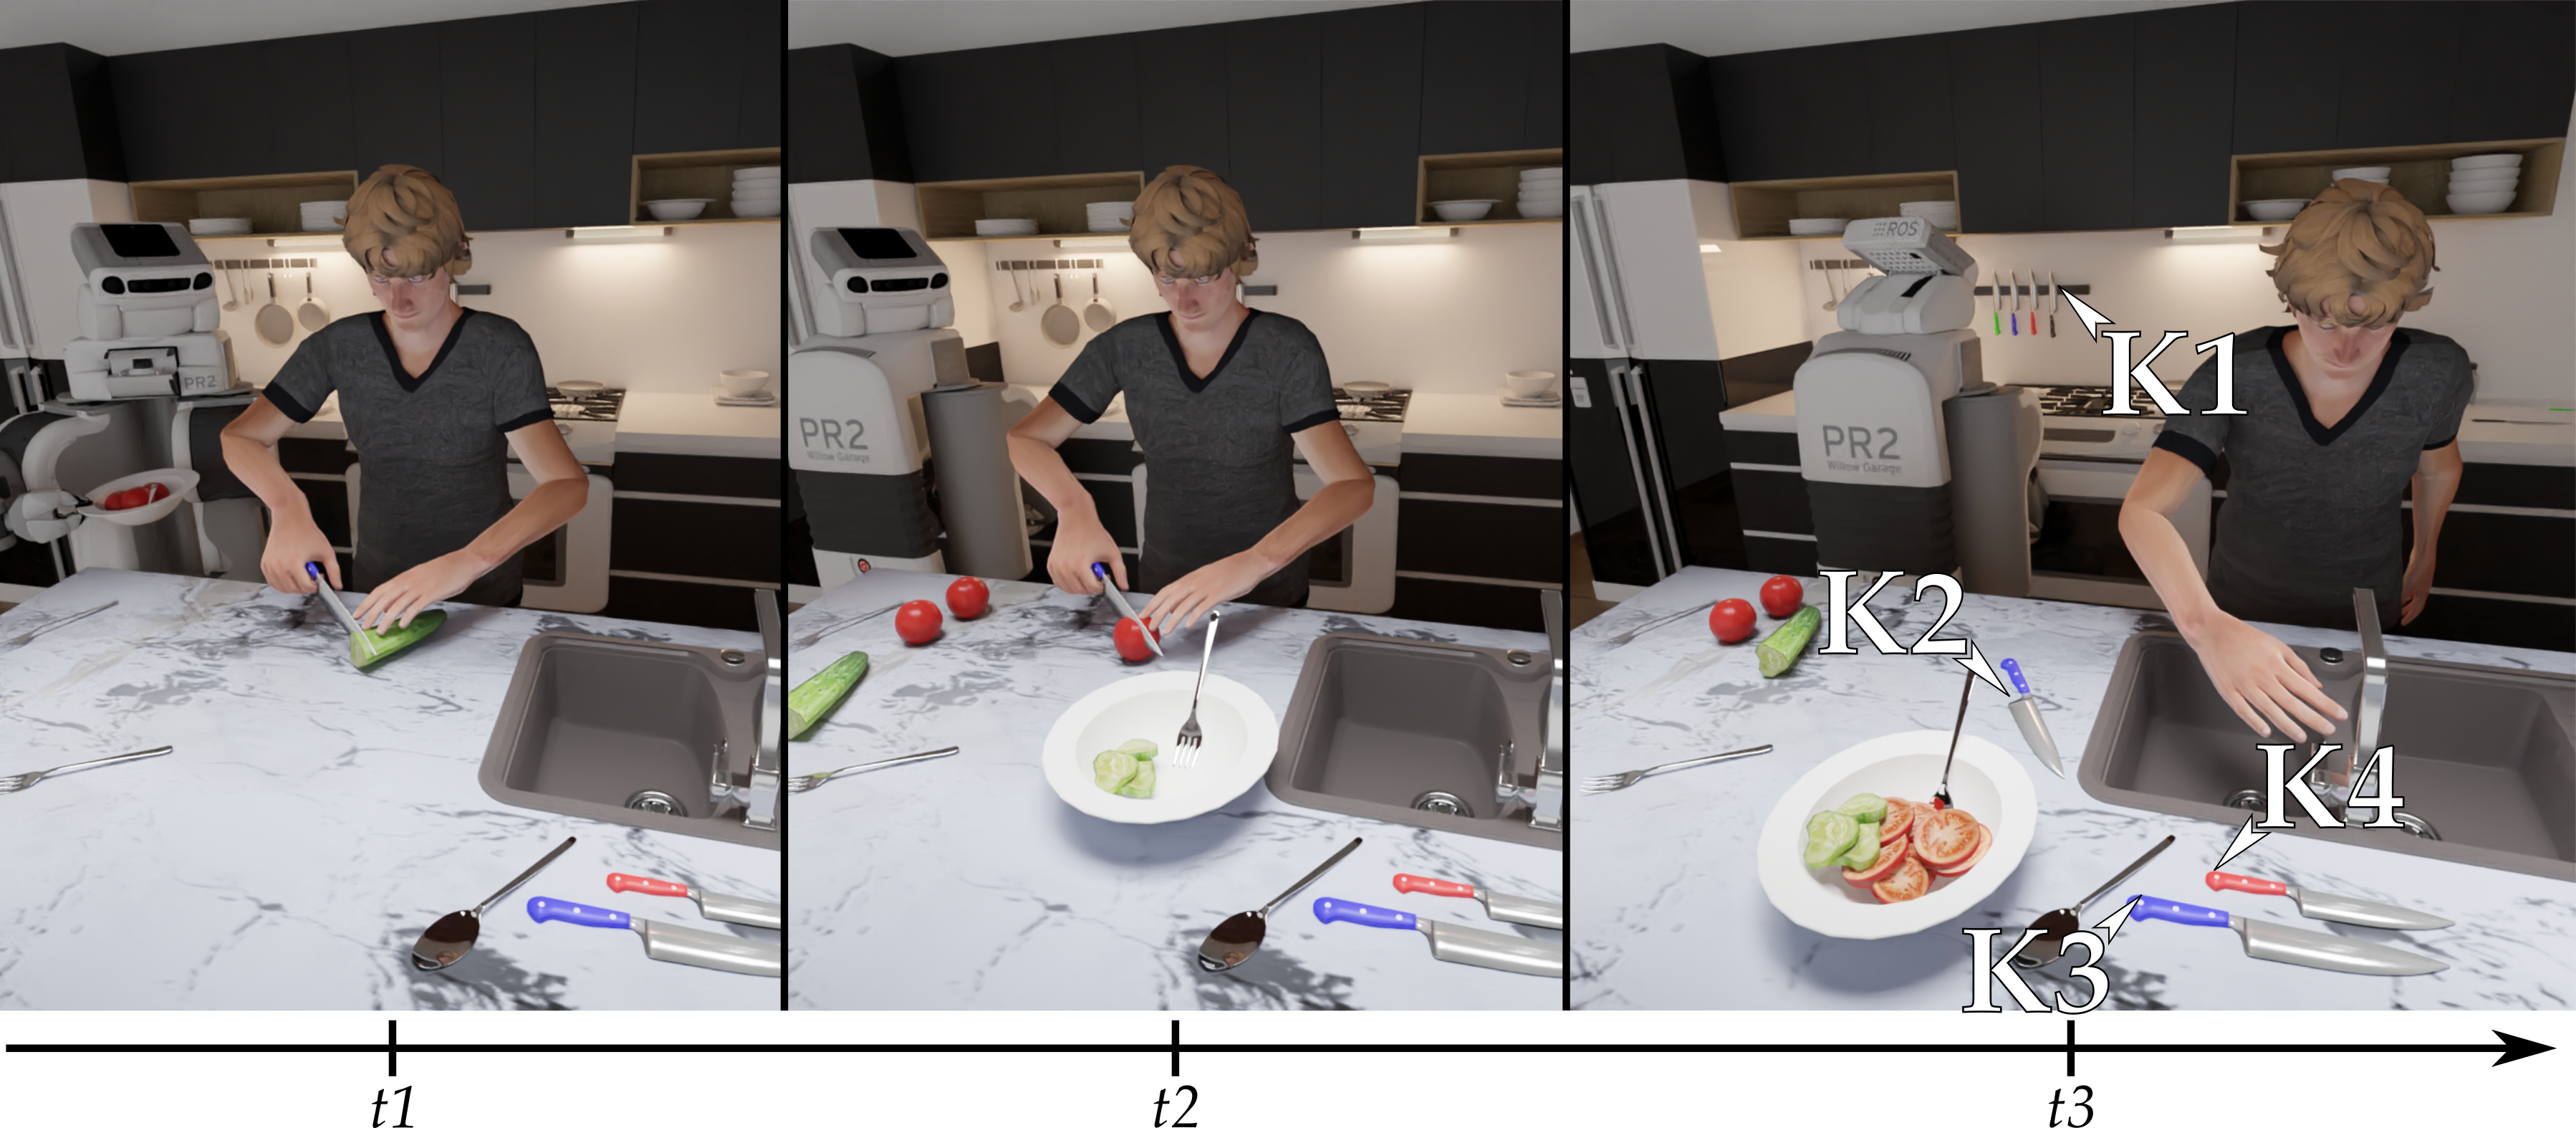
\includegraphics[width=\textwidth]{figures/chapter6/intro/intro.png}
\caption{\label{fig:chap6_intro} Referring to knife \textit{k2} in the current situation (\textit{t3}) is impossible if the robot is performing an action that does not allow it to see what is in front of the human. Considering a previous steps of the human's task, the robot can refer to the knife through the action to cut a tomato (\textit{t2}) or to cut a cucumber (\textit{t1}).}
\end{figure}

Consider the caption of the of an interaction represented in Figure~\ref{fig:chap6_intro} at the current instant \textit{t3}. The robot, in the back of the kitchen, has to ask the human for the knife \textit{k2}. Since the robot is performing another action of the joint task, it cannot see what is in front of the human. Consequently, it can know and thus use any spatial relations about \textit{k2}\footnote{We could also consider an object known by the robot but for which it does not have any information regarding its new location and searching for it. It would have to refer to it, to ask for the human help, without the possibility to use spatial relations.}. Therefore, the robot can only use \textit{k2} attributes (i.e. only it's color) to generate an expression referring to it. Still considering only the current instant \textit{t3}, two others blue knives hold in the kitchen being \textit{k1} and \textit{k3}. The knife \textit{k1} is attached to the wall in front of the robot meaning that it is already accessible to it and not to the human. This knife can thus be considered as being out of context and not leading to any ambiguity with \textit{k2}. The other blue knife \textit{k3} remains ambiguous since it does not have any perceptible attribute that differs from the one the robot has to refer to.

Until now, we only have considered the current situation \textit{t3} and not the human-robot shared experience about the task they perform. In the previous instant \textit{t2} the human was cutting a tomato with the knife \textit{k2}. At this previous instant, it was manifest to the human that the robot was observing the scene while he acted. This new information about the performed action could thus be used by the robot to generate a reference to the wanted knife in the current situation. A possible RE would be "\textit{the knife with which you cut the tomato}". 

Consider now the action a step before cutting the tomato at instant \textit{t1}. The human was cutting a cucumber with this same knife. The combination of these two past actions can be seen as the task of preparing vegetables. The robot can thus also use this knowledge to refer to the knife. A possible RE considering the totality of the interaction would be "\textit{the knife with which you prepared the vegetables}". The exploitation of shared knowledge about past activity in addition to the usual attributes and properties could lead to the generation of richer RE that could be easier to understand by the human partner. Besides, it allows extending REs use to contexts where the previous method was not effective.

This chapter is an extension of our previous work~\cite{buisan_2020_efficient} presented in chapter~\ref{chap:4}. It has been integrated within a cost-based Hierarchical agent-Base Task Planner to estimate the feasibility and cost of REs during the planning process~\cite{buisan_2020_human}, presented in chapter~\ref{chap:5}. In this chapter we will thus aim to create the inverse link, making the REG able to use execution traces resulting from the execution of hierarchical plans generated by HATP. Like the previous chapters, we only focus on the content determination of the REG problem but continue to consider the need to have names in natural language to enable linguistic realization.

The main contribution of this chapter is an extension of the ontology-based REG algorithm by \textbf{considering past agents' activities}. A side contribution of this chapter is a proposal of a formalism to \textbf{represent Hierarchical Execution Traces} (executed HTN-based plans) in an ontology. Our previous contribution considered cost functions based on the properties of the used relations to represent the cognitive load required for a human to interpret the RE. In this extension, we propose to add customizable cost functions based on time, to represent the cognitive load required for a human to remember referred activities.

First, we review the literature concerning HTN representation in ontologies and discuss REG-related works that not only consider caption of situations. Then, we describe the used knowledge bases and the usual structure of HTN and shared Hierarchical Execution Trace (HET). We then give in a first time an overview of how the knowledge bases should be updated and in a second time, the content of these updates in terms of how a shared Hierarchical Execution Trace (HET) is represented in an ontology. The extension of the algorithm is then detailed before ending with an efficiency comparison regarding the original version and a discussion around five illustrative cases to show the solutions found by our algorithm depending on the agent's knowledge about past activities.

\section{Related work}

In the previous chapter about Referring Expression Generation we already gave a good overview of the literature of the field. In this chapter, we thus briefly discuss few works trying to consider an interaction. We then move on to a wider part about the representation of HTN and execution traces in ontology to see the kind of information our algorithm could we to generate a new kind of referring expressions.

\subsection{Interaction based Referring expression}

\improvement{------more refs}
In all the previously presented works, the REG is only performed on the current environment state. Williams in~\cite{williams_2020_toward} is the first to add a temporal aspect by considering a sequence of REG. Like others before, he starts from the idea that to designate an entity it is preferable to use properties known by the hearer and that the latter will easily identify. Where others works, our included, represent that with cost on properties that we assume to be representative for the hearer, Williams tries to take advantage of an entire interaction. During such interaction, two partners will generate RE. The presented algorithm thus try to re-use properties used in previous descriptions made by the partner. In addition, he has implemented a forgetting model based on decay or interfering to avoid the use of properties used too long ago. This method has been tested on a "Guess Who"-style game. This kind of game has the advantage that the used properties hold between the REG and thus can be re-used. However, this assumption can no longer be maintained in a real dynamic interaction where objects are manipulated and their properties modified all along with the interaction.

Early in the field, Oberlander and Dale already showed that generating references to eventualities (\textit{i.e.} to past activities or past events) can be done in the same way as generating references to physical entities~\cite{oberlander_1991_generating}. However, they never generate references to entities through the use of past actions. To close this short tour, Wiriyathammabhum et al. in~\cite{wiriyathammabhum_2019_referring} use RE involving past actions to identify a referred entity in videos but does not generate them.

%The determination of the properties' costs will not be discussed here but we can mention \cite{belke_tracking_2002} and \cite{koolen_learning_2012} which use learning techniques to estimate the users' preferences.

\subsection{HTN-based tasks representation in ontology}

In robotic and even more in HRI, storing semantic information about past activities is needed to generate training data~\cite{diab_2020_knowing} and learn from experience~\cite{petit_2016_reasoning}, or to speak about what happened~\cite{mealier_2017_narrative}. Some approaches represent the past actions using structured sets of SQL tables~\cite{mealier_2017_narrative}, but such a representation lacks semantic information both on the involved entities (e.g. a robotic agent is a specific type of agent) and on the actions (e.g. a cut action is part of a salad preparation task). Since ontologies are fully suitable to represent semantic information about entities and their relations, they have been used to represent task planning knowledge. In~\cite{sun_2019_rtpo}, a Robot Task Planning Ontology (RTPO) is proposed but the model does not consider the rich semantics involved by the hierarchical nature and intricacies of human-robot joint activities. For example, they represent the fact that the action "ChargeAction" is a "ChargeTask" while a more correct semantic would be that the "ChargeTask" is composed of a "ChargeAction".

To represent episodes, the EASE-CRC has put forward the concept of narratively-enabled episodic memories(NEEMs)~\cite{diab_2020_knowing}. It is a log of perception events and sensor data annotated to give comprehensive logs of tasks performed by a robot. The annotations are based on the terminology provided by the Socio-physical Model of Activities(SOMA)~\cite{bessler_2020_foundations}. It proposes a high-level description of what s an event or an object in addition to the notion of plan. However, a plan is just a succession of actions and this terminology thus not support the use of HET for the moment. A design pattern for the representation of such NEEMs in ontology has been proposed in~\cite{bernd_2020_modelling}. However, this pattern is too cumbersome for ontology developers and not practical to use in side-fields we the safety of data input is not mandatory for the moment.

HTN is a very popular way for representing, planning, and controlling autonomous agents' activities \cite{ghallab_2004_automated, ingrand_2017_deliberation}. It is a tree representing how to decompose abstract tasks into primitive tasks directly applicable by an agent \cite{erol_1994_htn}. They are widely used for robotic planning as they allow to efficiently find complex plans by choosing between different task decompositions depending on the world state. 
Unlike more classical state-space search-based planning algorithms like STRIPS~\cite{fikes_1971_strips}, HTN planning does not explore applicable actions until a goal is reached, but rather tries to fully decompose an abstract task into applicable primitive tasks. Moreover, HTN planning is often quicker as domains (HTN representations) are provided with expert knowledge through the hierarchical structure and task decomposition alternatives. 
In HRI scenarios, their usefulness is even more apparent. In \cite{lallement_2014_hatp}, an HTN is used to generate human-robot joint plans. Furthermore, the hierarchical structure can be used to negotiate or communicate high-level plans when details do not matter~\cite{milliez_2016_using}. As an example, for a robot equipped with a charge plug and solar panels, an HTN may represent the abstract task of "ChargeTask" as being decomposed into either "GoToChargeStation" primitive (or abstract) task or "GoOutside" task. An HTN planner would then explore these alternatives and generate the most appropriate plan depending on the current world state: here the current weather.

To the best of our knowledge, few works exist on the representation of an HTN and their Hierarchical Execution Trace (HET) in ontologies. Umbrico et al. in~\cite{umbrico_2020_ontology} describe the notion of complex tasks composed of simple tasks but does not go further in the representation. In \cite{freitas_2014_using} only the planning domain is represented. The major issue is that the ontology classes are used to describe the general HTN concepts (i.e. action, method) while the field concepts (e.g. the cut task in our example) are described using the ontology individuals. Hence, this representation does not allow to represent abstracts or primitives tasks instantiations. This distinction between the domain as a high-level knowledge and thus represented in the ontology classes and properties and the HET representation as an instantiation of a domain is important to us. It allows to both represent how a given task could be done and how it has been done during execution. Our work is closer to BOWL~\cite{ko_2011_business}, an HTN ontology for business process representation. Even if they have defined some specific relations for the Business-to-Business field, the general tasks, decomposition, and tasks links representation are interesting. However, BOWL only represents the HTN and not HETs, but does not preclude it.

\section{Structuring and gathering the knowledge}

\subsection{The three used knowledge representation}

\subsubsection{The Hierarchical Task Network}

\subsubsection{The semantic knowledge base}

\subsubsection{The episodic knowledge base}

\subsection{The knowledge gathering scheme}

\subsection{Building the ontology}

\subsubsection{HTN in ontology}

\subsubsection{HET in ontology}

\section{Modifying the REG algorithm to support the past experiences}

\section{Results}

\subsection{One execution trace for five reffering expressions}

\subsection{The impact of the extention on the performances}

\section{Adapting the verbalization algorithm}